\documentclass[12pt]{article} % Set font size to 12 and set document type
\usepackage[procnames]{listings} % Code highlight
\usepackage{xcolor}
\usepackage{array}
% \definecolor{code_bg}{rgb}{0.95,0.95,0.92}
% \definecolor{code_green}{rgb}{0,0.6,0}
% \definecolor{code_gray}{rgb}{0.5,0.5,0.5}
% color def
\definecolor{keywords}{RGB}{255,0,90}
\definecolor{comments}{RGB}{0,0,113}
\definecolor{red}{RGB}{160,0,0}
\definecolor{green}{RGB}{0,150,0}
 
\lstset{language=Python, 
        basicstyle=\ttfamily\small, 
        keywordstyle=\color{keywords},
        commentstyle=\color{comments},
        stringstyle=\color{red},
        showstringspaces=false,
        identifierstyle=\color{green},
        procnamekeys={def,class}}
\usepackage{geometry}
\geometry{letterpaper, portrait, margin=1in} % Set document layout
\usepackage{graphicx} % Needed to import images
% \usepackage{indentfirst} % Enable the first paragraph to be indented
\renewcommand{\familydefault}{\sfdefault} % Set document fonts to sans-serif
\setlength{\parindent}{30pt} % Set indent size


\begin{document}

\begin{flushright}
        WO1 Jik Oh\\
        OOP: dungeon dudes\\
        2023.10.25\\
\end{flushright}

\begin{center}
        {\huge Design Plan Document}
\end{center}

\section{Requirements}

The requirements for this project include:


\begin{itemize}
        \item Create a Rogue class
        \item Rogue will have following Stat Growth
\end{itemize}

\begin{footnotesize}
\begin{center}
\begin{tabular}{ | m{3cm} | m{1cm} | m{1cm} | m{8cm} |  }
\hline
Stat & Initial & Per Level & Description \\
\hline
Hit Points & 75 & 18 & Health Points \\
\hline
Strength & 10 & 1 & Strength translates to attack power at 1 strength = 1 attack power. Directly increases the damage of Ambush. \\
\hline
Agility & 12 & 2 & Agility translates to attack power at 1 agility = 1 attack power and defense power at 2 agility = 1 defense power. Also decreases the chance you'll surprise attacked in battle. Directly increases the damage of Ambush. \\
\hline
Intelligence & 5 & 1 & Directly increases the damage of Rogue poisons. \\
\hline
Luck (special) & 1 & 1/2 & Luck can empower Rogue abilities \\
\hline
Experience & 0 & 35x\textsuperscript{2} & Rogue progress levels faster than average \\
\hline
\end{tabular}
\end{center}
\end{footnotesize}

\begin{itemize}
    \item Rogue Equipment will be
\end{itemize}

\begin{footnotesize}
\begin{center}
\begin{tabular}{ | m{2cm} | m{2cm} | m{10cm} | }
\hline
Slot & Types & Expected Stats \\
\hline
Weapon & Dagger & Rogue Weapons have attack power equal to approximately their level. They also have a modifier approximately equal to their level which modifies all Physical damage dealt. Weapons over level 10 have a modifier approximately equal to half their level to which modifies all Poison damage dealt. They have a chance to additional bonus attack power of approximately half their level.\\
\hline
Armor & Medium & Rogue Armors have defense power equal to approximately their 0.85 times their level +8. They have defensive modifiers to 2 damage types. They have a chance to have additional bonus defense power or attack power of approximately half their level. Armor defensive modifiers have approximately 20 + (level *2) modification value across both stats.\\
\hline
Accessory & Thieves Tools & The Rogues Accessory are Thieves Tools. Thieves Tools have attack power equal to approximately 0.75 * level + 10 of their level and defensive modifiers to 2 damage types. Thieves Tools use the same defensive modifier scaling as Armor. Thieves Tools sometimes have additional Physical or Poison damage modifiers equal to approximately 30\% of their level or a defensive modifier for Physical Damage equal to approximately their half their level + 10.\\
\hline
\end{tabular}
\end{center}
\end{footnotesize}

\begin{itemize}
    \item Rogue will have following skills
\end{itemize}

\begin{footnotesize}
\begin{center}
\begin{tabular}{ | m{3cm} | m{1.5cm} | m{10cm} | }
\hline
Skill & Level & Description \\
\hline
Attack & 1 & Rogue attacks deal damage with a base of their attack\_power. \textbf{Empower}: Attack Empowered with luck always deal their maximum damage as base damage. \\
\hline
Luck & 1 & Rogue uses a Luck point to empower their next ability. Using Luck does not pass the Rogue’s turn.\\
\hline
Theives Tricks & 1 & \textbf{passive:} Rogues gain 30\% more gold from winning a battle.\\
\hline
Preparation & 3 & The Rogue analyzes the battlefield, gaining 10 to their Physical and Poison damage modifiers, and coating their weapon in poison. Adding additional Poison damage to each attack which deals Physical damage (base Poison damage done equal to intelligence). Increase damage modifier adjustments by 5 if the Rogue’s weapons are already coated in poison. \textbf{Empower:} Preparation also Identifies the enemy. \\
\hline
Healing Potion Affinity & 5 & \textbf{passive:} Using a Healing\_Potion during combat also gives the Rogue time to coat their weapon in poison. Rogues have a percentage chance equal to their level * 1.5 to find a Healing\_Potion after winning a battle. \\
\hline
Surprise Attack & 8 & \textbf{passive:} The first Attack each turn a Rogue does deals 50\% increased damage and lowers the enemies Poison defensive modifier by an amount equal to the Rogue’s level.\\
\hline
Evasion & 10 & Rogue has a 50\% chance to avoid 100\% of the damage from the next two events which would cause the Rogue 1 or more damage. \textbf{Empower:} Evasion has a 10\% additional chance to avoid 100\% of the damage and lasts 1 additional damage event. \\
\hline
Ambush & 13 & \textbf{Once per Battle:} Rogue attacks for damage equal to Attack Power + Agility + Strength.  Ambush can consume Surprise Attack. \textbf{Empower:} Ambush does its maximum damage as base damage deals x3 the normal poison damage if weapons are coated in poison. \\
\hline
Increase Luck & 17 & Deal an attack which does 70\% normal damage, the Rogue gains 1 Luck point, up to their maximum. \\
\hline
Auto-Potion & 20 & \textbf{passive:} Rogues automatically consume a Healing\_Potion on their first action in combat. If the Rogue is at maximum hit points, no "Healing\_Potion" is consumed but the Rogue gains all other benefits of Healing Potion Affinity \\
\hline
Enhanced Abilities & 25 & \textbf{passive:} Base modifier adjustment of Preparation is increased to 20, Surprise Attack now increases damage 75\%, Evasion has a base avoidance chance of 60\% and lasts for 3 damage events. Ambush now deals additional damage equal to the Rogue’s agility, Increased Luck now does 85\% of Normal Damage.\\
\hline
Damage/Variance & Physical, Poision & Rogues only do Physical damage with their attacks with additional Poison damage if their weapons are coated in poison. All Rogue variance is the base damage normally distributed 8\% of the base damage with a standard deviation of 4\% of the base damage, up to 24\% additional damage + max(0, min(base*.24,random.gauss(base*.08, base*.04))). Equipment variance follows the same formula as Fighter variance. \\
\hline
\end{tabular}
\end{center}
\end{footnotesize}

\begin{itemize}
    \item Source codes for Rogue class should produce no warnings or errors with pycodestyle
    \item Playing the game with Rogue class should not make the program crash or fall into an infinite loops
\end{itemize}

\section{Architecture}

\subsection{Overview}

The example Fighter class gave a lot of insights on how to construct a playable class. Most of passive skills will utilize flag variables within the class. All special attack skills will have their own functions.

\subsubsection{Class Variables}
Rogue class will have following additional and class exclusive variables to account for all skills.

\begin{lstlisting}[language=Python]
    self._empowered: bool = False
    self._poison_coated: bool = False
    self._surprise_attack_left: bool = True
    self._ambush_left: bool = True
    self._evasion_active: bool = False
    self._evasion_count: int = 0
    self._evasion_chance: int = 0
    self._auto_potion_active: bool = False
    self._first_action: bool = True
    self._enhanced_abilities_on: bool = False
\end{lstlisting}

\subsubsection{Class Methods}
All of Rogue active skills will have their own functions as class methods. Followings will be Rogue class exclusive methods. 
\begin{itemize}
        \item luck: Consume special and turn empowered flag on
        \item preparation: return Battle Cry for physical and poison
        \item use\_healing\_potion: This method should be overwritten due to the Healing Potion Affinity Passive. 
        \item evasion: Set evasion flag with apporpriate count and chance
        \item ambush: Once executed, change ambush flag to remove the skill from the list
        \item increase\_luck: Increase special by 1 and attack the enemy
        \item auto\_potion: gets called on every special attacks and normal attack first, set the flag off once succesfully executed
\end{itemize}

\newpage

\section{Class Diagram}
\begin{figure}[htp]
    \centering
    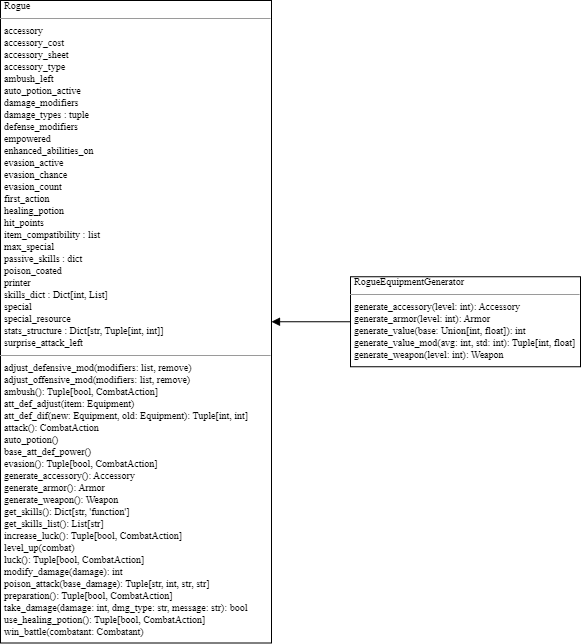
\includegraphics[width=0.9\linewidth]{images/rogue_diagram.png}
\end{figure}
\end{document}
